%-----------------------------------------------------------------
% Rodrigo Chang, 2019
% Banco de Guatemala
% Programa de Estudios Superiores 2019-2020
% Diapositivas del curso "Programación I"
%
% Descargo de responsabilidad.
%   El contenido de este documento es responsabilidad exclusiva de
% su(s) autores. Cualquier opinión expresada no necesariamente
% representa la postura institucional del Banco de Guatemala. 
% 
% Contenido.
%   El contenido de estas diapositivas está construido a partir de 
% modificaciones al material provisto por Ana Bell, Eric Grimson y 
% John Guttag para el curso 6.0001 Introduction to Computer Science 
% and Programming in Python, otoño 2016, Massachusetts Institute of 
% Technology: MIT OpenCourseWare, https://ocw.mit.edu
%
% Licencia: 
% Creative Commons BY-NC-SA
% https://creativecommons.org/licenses/by-nc-sa/4.0/.
%
% Formato. 
%   El formato utilizado para la elaboración de este documento 
% ha sido modificado a partir del repositorio: 
%       https://github.com/rinnert/statlearning-python-pwf
%
% Kurt Rinnert, 2019
%   Copying and distribution of this file, with or without 
% modification, are permitted in any medium without royalty provided 
% the copyright notice and this notice are preserved. This file is 
% offered as-is, without any warranty.
%
%-----------------------------------------------------------------
\documentclass[mathserif]{beamer}
% Para configurar las diapositivas en relación 16:9, 
% agregar la opción aspectratio=169

% Título de la presentación y tópicos a tratar
\usepackage{arev, arevmath}
\usepackage[scaled]{cabin}
%\usepackage[T1]{fontenc}
\usepackage[super]{nth}
\usepackage{pifont}
\usepackage{wasysym}
\usepackage{tabularx}
\usepackage{array}
\usepackage{booktabs}
\usepackage{boldline}
\usepackage{colortbl}
\usepackage{amsmath}
\usepackage{bm}
\usepackage{tcolorbox}
\usepackage{adjustbox}
\usepackage{minibox}
\usepackage{makecell}
\usepackage{adjustbox}
\usepackage{textcomp}
\usepackage[absolute,overlay]{textpos}
\setlength{\TPHorizModule}{1mm}%
\setlength{\TPVertModule}{1mm}%
\tcbuselibrary{skins}
\usepackage{graphicx}
\usepackage[spanish, es-tabla]{babel}
\usepackage[utf8]{inputenc}
\usepackage{csquotes}

\usepackage{comment}
\usepackage{svg}

\usepackage{verbatim}
\usepackage{pdfpages}

% Columnas múltiples
\usepackage{multicol}

% -------------------------------------------
%	LISTINGS
% -------------------------------------------
% Paquetes necesarios para los códigos
\usepackage{listings}
\usepackage{color}
% Configuración de listings (pendiente)
%\input{conf/listingStyles}
% Redefinición de titulos de caption
\renewcommand\lstlistingname{\textbf{Código}}
\renewcommand\lstlistlistingname{Códigos}

% Definición de colores para Python (Jupyter notebooks)
\definecolor{python_keyword_color}{RGB}{0, 128, 0}
\definecolor{python_string_color}{RGB}{186, 34, 34}
\definecolor{python_comment_color}{RGB}{1, 121, 121}
\definecolor{frame_numbers_color}{rgb}{0.5,0.5,0.5}
\definecolor{python_identifier_color}{RGB}{0,0,0}
\definecolor{jupyter_background}{RGB}{247, 247, 247}
\definecolor{jupyter_frame}{RGB}{207, 207, 207}

% Definicion de estilo para Python
\lstdefinestyle{custom_python}{
	language=python,			% the language of the code
	backgroundcolor=\color{jupyter_background}, 
	% the size of the fonts that are used for the code
	basicstyle=\linespread{1}\small\ttfamily,	
	% Configuración de colores
	commentstyle=\color{python_comment_color},	% comment style
	identifierstyle=\color{python_identifier_color},
	keywordstyle=\mdseries\color{python_keyword_color},	% keyword style
	numberstyle=\tiny\color{frame_numbers_color},	
	stringstyle=\color{python_string_color}, % string literal style 
	captionpos=t,				% sets the caption-position to bottom
	breakatwhitespace=false,	% sets if automatic breaks should only happen at whitespace
	breaklines=true,			% sets automatic line breaking
	morekeywords={},			% if you want to add more keywords to the set
	deletekeywords={eps},		% delete keywords from the given language
	escapeinside={\%*}{*)},		% if you want to add LaTeX within your code
	framesep=3pt,
	keepspaces=true,			% keeps spaces in text,       
	numbers=none, 	% (none, left, right)
	numbersep=5pt,	% how far the line-numbers are from the code
	% if not set, the frame-color may be changed on line-breaks within not-black text (e.g. comments (green here))
	rulecolor=\color{jupyter_frame}, 
	% show spaces everywhere adding particular underscores; it overrides 'showstringspaces'
	showspaces=false,                
	% underline spaces within strings only
	showstringspaces=false,          
	% show tabs within strings adding particular underscores
	showtabs=false,                  
	stepnumber=0,	% the step between two line-numbers      
	% sets default tabsize to 2 spaces
	tabsize=2,                       
	% lets you use non-ASCII characters; for 8-bits encodings only, does not work with UTF-8
	extendedchars=true,      
	% Support additional characters            
	literate=
  {á}{{\'a}}1 {é}{{\'e}}1 {í}{{\'i}}1 {ó}{{\'o}}1 {ú}{{\'u}}1
  {Á}{{\'A}}1 {É}{{\'E}}1 {Í}{{\'I}}1 {Ó}{{\'O}}1 {Ú}{{\'U}}1
  {à}{{\`a}}1 {è}{{\`e}}1 {ì}{{\`i}}1 {ò}{{\`o}}1 {ù}{{\`u}}1
  {À}{{\`A}}1 {È}{{\'E}}1 {Ì}{{\`I}}1 {Ò}{{\`O}}1 {Ù}{{\`U}}1
  {ä}{{\"a}}1 {ë}{{\"e}}1 {ï}{{\"i}}1 {ö}{{\"o}}1 {ü}{{\"u}}1
  {Ä}{{\"A}}1 {Ë}{{\"E}}1 {Ï}{{\"I}}1 {Ö}{{\"O}}1 {Ü}{{\"U}}1
  {â}{{\^a}}1 {ê}{{\^e}}1 {î}{{\^i}}1 {ô}{{\^o}}1 {û}{{\^u}}1
  {Â}{{\^A}}1 {Ê}{{\^E}}1 {Î}{{\^I}}1 {Ô}{{\^O}}1 {Û}{{\^U}}1
  {œ}{{\oe}}1 {Œ}{{\OE}}1 {æ}{{\ae}}1 {Æ}{{\AE}}1 {ß}{{\ss}}1
  {ű}{{\H{u}}}1 {Ű}{{\H{U}}}1 {ő}{{\H{o}}}1 {Ő}{{\H{O}}}1
  {ç}{{\c c}}1 {Ç}{{\c C}}1 {ø}{{\o}}1 {å}{{\r a}}1 {Å}{{\r A}}1
  {€}{{\EUR}}1 {£}{{\pounds}}1,   
}

% Configurar el listing para el documento actual
\lstset{
	style = custom_python, 
	frame = single
}

% -------------------------------------------
%	OTRAS CONFIGURACIONES
% -------------------------------------------
\makeatletter
\newcommand{\antsize}{\@setfontsize{\antsize}{4pt}{4pt}}
\makeatother
\newcommand{\at}{\makeatletter @\makeatother}

\newcommand{\cmark}{\ding{51}}%
\newcommand{\bottomline}[1]{\vskip0pt plus 1fill{\alert{#1}\phantom{g}\vskip 1.0mm}}

% Rutas para las imágenes
%\graphicspath{{figs/}{figs/common/}}

% Separación de filas en las tablas más amplia
\renewcommand{\arraystretch}{1.2}


% -------------------------------------------
%	ESTILO DE LA PRESENTACIÓN
% -------------------------------------------

\mode<presentation>%
{
	\usetheme{default}
	%\usetheme[width=2.5cm]{PaloAlto}
	\usecolortheme{dove}
	\useoutertheme{infolines}
	% oder auch nicht

	% BANGUAT Colors
	\definecolor{BANGUATblue}{RGB}{37,86,162} % 0x255682
	\definecolor{BANGUATorange}{RGB}{255,130,0} % 0xff8200
	\definecolor{BANGUATgreen}{RGB}{0,100,0}
	\definecolor{BANGUATdark}{RGB}{80,80,80} % 0x505050
	\definecolor{BANGUATlight}{RGB}{120,120,120}
	\definecolor{BANGUATbrown}{RGB}{178,91,0}

	\definecolor{codebg}{rgb}{0.95,0.95,0.95}

	% Color theme
	\setbeamercolor{alerted text}{fg=BANGUATorange}
	\setbeamercolor{frametitle}{fg=BANGUATblue}
	\setbeamercolor{title}{fg=BANGUATblue}
	\setbeamercolor{subtitle}{fg=BANGUATorange}
	\setbeamercolor{normal text}{fg=BANGUATdark}
	\setbeamercolor{author in foot}{fg=BANGUATblue}
	\setbeamercolor{item}{fg=BANGUATblue}
	\setbeamercolor{footline}{fg=BANGUATblue}
	%\setbeamercolor{item projected}{bg=BANGUATorange}
	%\setbeamercolor{item projected}{fg=white}

	\setbeamertemplate{headline}
	{}
	\setbeamertemplate{frametitle}
	{
		%\textbf{{\insertframetitle\phantom{g}}}\\
		%\textbf{\insertframetitle\phantom{g}}\\
		\textbf{\underline{\insertframetitle\phantom{g}}}\\
		%\textbf{\underline{\insertframetitle}}\\
		\vskip 1.0mm
		%{\color{UOLgold}\hrule height 2pt}
		%\par
	}
	\addtobeamertemplate{frametitle}{}{\vspace{-1em}}
	\setbeamertemplate{footline}{
		{%
			\textbf{ \hskip 3.0mm\insertshorttitle\phantom{.}---\phantom{.}\insertshortinstitute\hfill\insertframenumber\,/\,\inserttotalframenumber\hskip 3.0mm} 
		}
	}

	\setbeamertemplate{navigation symbols}{}%remove navigation symbols
	\setbeamertemplate{itemize items}[circle]
	\setbeamertemplate{enumerate items}[fg=BANGUATblue]
	\setbeamercolor{itemize items}{fg=BANGUATblue}
	\setbeamercolor{sidebar}{bg=BANGUATblue}
	\setbeamercolor{title in sidebar}{fg=BANGUATorange}
	\setbeamercolor{author in sidebar}{fg=BANGUATorange}
	\setbeamercolor{section in sidebar}{fg=BANGUATorange}
}



% -------------------------------------------
%	CONFIGURACIÓN DE DIAPOSITIVA DE TÍTULO
% -------------------------------------------

% Título del curso
\title[Programación I]{\textbf{%
Introducción a las ciencias de la computación\\%
{\it y programación en Python}}\\%
%\href{https://ocw.mit.edu/courses/electrical-engineering-and-computer-science/6-0001-introduction-to-computer-science-and-programming-in-python-fall-2016/}{\tiny\it Basado en el curso ``Introduction to Computer Science and Programming in Python'' por Ana Bell, Eric Grimson, y John Guttag.}%
\vspace{3em}%
}
%\vspace{-2.5cm}{}

% Autor y correo electrónico
\author{\href{mailto:?to=Rodrigo Chang <rrcp@banguat.gob.gt>&subject=PES Programación I}{Rodrigo Chang}}

% Información del instituto
\institute[\href{https://www.banguat.gob.gt/}{Banco de Guatemala}]%
{\color{BANGUATblue} \bfseries \href{https://www.banguat.gob.gt/}{Banco de Guatemala}\\%
\vspace{3mm}%

\includegraphics[width=0.13\textwidth]{figs/common/logo-banguat.png}}

% Sin fecha en particular
\date{}

% Información de licencias y copyright
\titlegraphic{
	 %\texorpdfstring{\vspace{-3cm}}{}
	 \vspace{-1.5cm}
	 \begin{minipage}[b][1cm][b]{0.25\textwidth}%
	    \color{BANGUATlight}\antsize
		%Copyright \textcopyright~2019\\
		\href{mailto:?to=Rodrigo Chang <rrcp@banguat.gob.gt>&subject=PES Programación I}{Rodrigo Chang <rrcp@banguat.gob.gt>}\\
		Este material está construido a partir de modificaciones al material provisto por Ana Bell, Eric Grimson y John Guttag para el curso \textit{6.0001 Introduction to Computer Science and Programming in Python}, otoño 2016, Massachusetts Institute of Technology: MIT OpenCourseWare, \href{https://ocw.mit.edu}{https://ocw.mit.edu}. Licencia: \href{https://creativecommons.org/licenses/by-nc-sa/4.0/}{Creative Commons BY-NC-SA}.
		
		%Copying and distribution of this file, with or without modification, are permitted in any medium without royalty provided the copyright notice and this notice are preserved.  This file is offered as-is, without any warranty.


		%Some of the figures in this presentation are taken from ``An Introduction to Statistical Learning, with applications in R''  (Springer, 2013) with permission from the authors: G. James, D. Witten,  T. Hastie and R. Tibshirani 
	 \end{minipage}%
	 \hspace{9cm}
}

% Restar uno al contador
\addtocounter{framenumber}{-1}

% Cajas de colores
\newcommand{\tabboxset}{\tcbset{enhanced, nobeforeafter, boxrule=0pt, boxsep=0pt, colback=codebg, colframe=codebg, coltext=BANGUATdark, rounded corners, arc=4pt, fonttitle={\bfseries\tiny}}}
\newcommand{\codeboxset}{\tcbset{enhanced, nobeforeafter, boxrule=0pt, boxsep=0pt, colback=codebg, colframe=codebg, coltext=BANGUATdark, rounded corners, arc=4pt, fonttitle={\bfseries\tiny}}}

% Comandos útiles
\newcommand{\orange}{\color{BANGUATorange}}
\newcommand{\blue}{\color{BANGUATblue}}
\newcommand{\dark}{\color{BANGUATdark}}
\newcommand{\R}{\mathbb{R}}
\newcommand{\dat}[1]{{\footnotesize\tt\orange #1}}
\newcommand{\mdat}[1]{\text{\dat{#1}}}
\newcommand{\val}[1]{{\footnotesize\tt\blue #1}}
\newcommand{\mval}[1]{\text{\val{#1}}}
\newcommand{\e}[1]{\emph{#1}}
\newcommand{\bh}{\hat{\beta}}
\newcommand{\h}{\hat}
\newcommand{\bl}{\bottomline}


\makeatletter
\newcommand{\includegraphicsdpi}[3]{%
	\pdfimageresolution=#1%
	\includegraphics[#2]{#3}%
	\pdfimageresolution=72%
}

\newcommand{\Quote}[2]{%
	\begin{center} 
		\begin{minipage}{0.7\textwidth} 
			\hrule
			\vskip 3mm
			\emph{{\color{BANGUATblue} ``#1''}\\
			{\color{BANGUATorange} --- #2}}
			\vskip 3mm
			\hrule
			\vskip 2mm
		\end{minipage}
	\end{center}
}

% Texto centrado en la diapositiva, quizás para el abstract o para indicar abajo de un quote
\newenvironment{blurb}%
	{\begin{center}\begin{minipage}{0.6\textwidth}\footnotesize}
	{\end{minipage}\end{center}}

% Environment para códigos o algoritmos. Parecido a un bottomline, se puede utilizar para dar definiciones o enfatizar en algún concepto
\newenvironment{cpage}%
	{\begin{center}\begin{minipage}{0.75\textwidth}}
	{\end{minipage}\end{center}}

% Bloque (similar a un pop-up) de alerta para indicar resultados en tablas, definiciones, fórmulas, etc.
% Primer argumento es el tamaño 
% Segundo argumento es el título del bloque
\newenvironment{popblock}[2]%
	{\begin{center}\begin{minipage}{#1}\footnotesize
		\begin{tcolorbox}[colframe=codebg, colback=white, colupper=BANGUATdark, title={\normalsize\bfseries\blue #2}]}
	{\end{tcolorbox}\end{minipage}\end{center}}
\makeatother

% Incluir diapositivas en PDF
% 1 - Título de la diapositiva
% 2 - páginas del PDF a incluir
% 3 - ruta hacia el archivo PDF
\newcommand{\includeslides}[3]{%
{%
\setbeamercolor{background canvas}{bg=}%
\addtocounter{framenumber}{1}%
\includepdf[pages={#1}, link=true, pagecommand={%
\Large\blue\bfseries\underline{%
#3\phantom{g}}%
\vspace{-1em}%
\vskip 1.0mm}]{#2}%
}}
\subtitle{%
  \bfseries{Diccionarios y recursión}\\%
  %{\tiny\it Manejo de strings, \textit{guess and check}, métodos de aproximación}\\%
}

% Inicio del documento
\begin{document}
\frame[plain]{
	%\vskip 1.0mm
	\titlepage
	%\vskip 1.0mm
}
%-----------------------------------------------------------------
% Empieza el contenido de la presentación
%-----------------------------------------------------------------

\begin{frame}{Abstract}
	\Quote{Talk is cheap. Show me the code.}{Linus Torvalds}
    
	\begin{blurb}
		Veremos un nuevo tipo {\blue compuesto} en Python: los diccionarios.
		
		Hablaremos del concepto de recursión y veremos sus aplicaciones.
		
	\end{blurb}
\end{frame}


\section{Diccionarios}

\begin{frame}[fragile]{Diccionarios - almacenar información}
    \begin{itemize}
        \item Supongamos que queremos guardar información de estudiantes de esta forma:
\begin{lstlisting}
names = ['Ana', 'John', 'Denise', 'Katy']
grade = ['B', 'A+', 'A', 'A']
course = [2.00, 6.0001, 20.002, 9.01]
\end{lstlisting}

        \item Utilizamos una {\blue lista diferente} para cada elemento.
        \begin{itemize}
            \item Cada lista debe ser del mismo {\blue largo}.
        \end{itemize}
        
        \item Cada índice se refiere a la información de la misma persona.
    \end{itemize}
\end{frame}

\begin{frame}[fragile]{Diccionarios - consultar información}
    \begin{itemize}
        \item Veamos esta función para obtener la información de \lstinline|student|:
\begin{lstlisting}
def get_grade(student, name_list, grade_list, course_list): 
    i = name_list.index(student)
    grade = grade_list[i]
    course = course_list[i]
    return (course, grade)
\end{lstlisting}

        \item Es {\blue\bfseries enmarañado} si se debe registrar mucha información diferente.
        
        \item Se deben mantener muchas listas.
        \item Siempre deben ser índices {\blue enteros}.
        \item Se debe recordar actualizar múltiples listas.
    \end{itemize}
\end{frame}

% Una manera más limpia, los diccionarios
\includeslides{43-45}{slides-60001/MIT6_0001F16_Lec6_mod.pdf}{Los diccionarios: una forma más limpia}

% keys and values
\begin{frame}[fragile]{Operaciones de diccionarios}
    \begin{itemize}
        \item \lstinline|grades.keys()| devuelve un iterable que actúa como una tupla de todas las llaves.
        \item \lstinline|grades.values()| devuelve un iterable que actúa como una tupla de los elementos almacenados.
    \end{itemize}
\begin{lstlisting}
grades = {'Ana':'B', 'John':'A+', 'Denise':'A', 'Katy':'A'}

grades.keys() # ['Denise','Katy','John','Ana']

grades.values() # ['A', 'A', 'A+', 'B']
\end{lstlisting}

\bottomline{El orden no está determinado en estas funciones.}
\end{frame}

% Acerca de las llaves y valores
\begin{frame}[fragile]{Llaves y valores}
    \begin{itemize}
        \item Valores: 
            \begin{itemize}
                \item De cualquier tipo ({\blue mutables} e {\blue inmutables}).
                \item Pueden ser {\blue duplicados}.
                \item Pueden ser listas o incluso otros diccionarios.
            \end{itemize}
            
        \item Llaves: 
            \begin{itemize}
                \item Deben ser {\orange\bfseries únicas}.
                \item Deben ser de tipos {\orange\bfseries inmutables}.
                \begin{itemize}
                    \item Cuidado con el tipo \lstinline|float| utilizado como llave.
                \end{itemize}
            \end{itemize}
         
        \item {\blue\bfseries No hay un orden} en las llaves o valores:
\begin{lstlisting}
d = {4:{1:0}, (1,3):"twelve", 'const':[3.14,2.7,8.44]}
\end{lstlisting}
    \end{itemize}
\end{frame}

% Listas vs diccionarios
\begin{frame}[fragile]{Listas vs. Diccionarios}
    \begin{columns}
        \begin{column}{0.5\textwidth}
        \begin{itemize}
            \item {\blue\bfseries Listas:}
            \item Secuencia {\blue ordenada} de elementos.
            \item Búsqueda de elementos por índice entero.
            \item Los índices tienen orden.
            \item Índice o llave de tipo \lstinline|int|.
            
        \end{itemize}
        \end{column}
        \begin{column}{0.5\textwidth}
        \begin{itemize}
            \item {\blue\bfseries Diccionarios:}
            \item {\orange\bfseries Asocian} una llave con un valor.
            \item Búsqueda de elementos a través de otros elementos.
            \item No existe un orden asociado.
            \item Llave o índice de tipo {\blue\bfseries inmutable}.
        \end{itemize}
        \end{column}
    \end{columns}
\end{frame}

% Agrergar aquí algún ejemplo o ejercicio de diccionarios
\begin{frame}[fragile]{Ejemplo: letras de canciones}
    \begin{enumerate}
        \item Crearemos un diccionario de frecuencias, es decir, una estructura de \lstinline|str:int|
        
        \item Encontraremos la palabra que más ocurre y cuántas veces.
        \begin{itemize}
            \item Utilizamos una lista, por si hay más de una palabra.
            \item Devolvemos una tupla \lstinline|(list, int)|.
        \end{itemize}
        
        \item Encontraremos las palabras que ocurren al menos $X$ veces.
        \begin{itemize}
            \item Permitimos al usuario escoger $X$ como parámetro.
            \item Devolvemos una listsa de tuplas, donde cada tupla es \lstinline|(list, int)|, conteniendo la lista de palabras ordenadas por frecuencia.
            \item Del diccionario, obtenemos la palabra más frecuente y borramos la entrada. Repetimos. Esto funciona porque estamos {\blue mutando} el diccionario de frecuencias.
        \end{itemize}
    \end{enumerate}
\end{frame}


\begin{frame}[fragile]{Diccionario de frecuencias}
\begin{lstlisting}
def lyrics_to_frequencies(lyrics):
    myDict = {}
    for word in lyrics:
        if word in myDict:
            myDict[word] += 1
        else:
            myDict[word] = 1
    return myDict
\end{lstlisting}
\end{frame}

\begin{frame}[fragile]{Utilizando el diccionario}
\begin{lstlisting}
def most_common_words(freqs):
    values = freqs.values()
    best = max(freqs.values())
    words = []
    for k in freqs:
        if freqs[k] == best:
            words.append(k)
    return (words, best)
\end{lstlisting}
\end{frame}

\begin{frame}[fragile]{Aprovechando el uso de diccionario}
\begin{lstlisting}
def words_often(freqs, minTimes):
    result = []
    done = False
    while not done:
        temp = most_common_words(freqs)
        if temp[1] >= minTimes:
            result.append(temp)
            for w in temp[0]:
                #remove word from dict
                del(freqs[w])  
        else:
            done = True
    return result
\end{lstlisting}
\end{frame}


\section{Recursión}

\begin{frame}[fragile]{¿Qué es recursión?}
    \begin{blurb}
    Es una forma en la cual se especifica un proceso basado en su propia definición.
    \end{blurb}
    \begin{itemize}
        \item Algorítmicamente: una forma de utilizar {\blue divide y conquistarás}.
        \begin{itemize}
            \item Reducir un problema a versiones más simples del mismo problema.
        \end{itemize}
        
        \item Semánticamente: técnica de programación donde una función {\blue\bfseries se llama a sí misma}.
        \begin{itemize}
            \item La meta es {\blue\bfseries no} tener recursión infinita.
            \item Deben existir {\blue\bfseries uno o más} casos base, simples de resolver.
            \item Debe permitir resolver el mismo problema con otras entradas para {\blue\bfseries simplificar} el problema más grande inicial.
        \end{itemize}
    \end{itemize}
\end{frame}

% Algoritmos iterativos
%\includeslides{7-8}{slides-60001/MIT6_0001F16_Lec6_mod.pdf}{Eficiencia: Fibonacci con diccionarios}
\begin{frame}[fragile]{Algoritmos iterativos}
    \begin{itemize}
        \item Las estructuras iterativas (ciclos \lstinline|while| y \lstinline|for|) llevan a los {\blue\bfseries algoritmos iterativos}.
        
        \item Capturan la computación en un conjunto de {\blue\bfseries variables de estado} que se actualizan en cada iteración del ciclo.
    \end{itemize}
    
    \begin{columns}
        \begin{column}{0.5\textwidth}
\begin{lstlisting}
def mult_iter(a, b): 
    result = 0
    while b > 0: 
        result += a
        b -= 1
    return result
\end{lstlisting}
        \end{column}
        \begin{column}{0.5\textwidth}
        \begin{itemize}
            \item El estado es capturado por la {\blue variable de iteración} \lstinline|i|. 
            \item El {\blue valor actual de la computación} es almacenado: \lstinline|result = result + a|.
        \end{itemize}
        \end{column}
    \end{columns}
\end{frame}

% Algoritmos recursivos
\begin{frame}[fragile]{Algoritmos recursivos}
   \begin{columns}
        \begin{column}{0.6\textwidth}
\begin{lstlisting}
def mult_recur(a, b):
    if b == 1:
        return a
    else:
        return a + mult_recur(a, b-1)
\end{lstlisting}
% Ecuaciones a*b
\[\begin{split}
    a * b & = \underbrace{a + a + \ldots + a}_{\text{$b$ veces}}\\
    ~ & = a + \underbrace{a + a + \ldots + a}_{\text{$b-1$ veces}}\\
    ~ & = a + a(b-1) 
\end{split}\]
        \end{column}
        \begin{column}{0.4\textwidth}
        \begin{itemize}
            \item {\orange\bfseries Paso recursivo:}
            \begin{itemize}
                \item ¿Cómo reducir el problema a una versión {\blue más simple / pequeña} del mismo problema?
            \end{itemize}
            
            \item {\orange\bfseries Caso base:}
            \begin{itemize}
                \item Seguir reduciendo el problema hasta obtener uno {\blue suficientemente simple} que pueda ser resuelto directamente.
                \item Cuando $b = 1$, $ab=a$
            \end{itemize}
        \end{itemize}
        \end{column}
    \end{columns}
\end{frame}

% Ejemplo de factorial
\begin{frame}[fragile]{Factorial}
    \begin{itemize}
        \item Recordemos que $n! = n*(n-1)*(n-2)*\ldots*1$.
\begin{lstlisting}
def factorial(n):
\end{lstlisting}     
        \item {\orange\bfseries Caso base:} ¿para qué caso conocemos el factorial?
\begin{lstlisting}
    if n == 1: 
        return 1
\end{lstlisting}
        
        \item {\orange\bfseries Paso recursivo:} escribimos el problema en términos de uno más simple {\blue para alcanzar el caso base}.
\begin{lstlisting}
    else: 
        return n * factorial(n-1)
\end{lstlisting}
    \end{itemize}
\end{frame}

\begin{frame}[fragile]{Factorial}
    \begin{itemize}
        \item \href{http://pythontutor.com/visualize.html#code=def%20fact%28n%29%3A%20%0A%20%20%20%20if%20n%20%3D%3D%201%3A%0A%20%20%20%20%20%20%20%20return%201%20%0A%20%20%20%20else%3A%0A%20%20%20%20%20%20%20%20return%20n*fact%28n-1%29%0A%20%20%20%20%20%20%20%20%0Aprint%28fact%284%29%29&cumulative=false&curInstr=9&heapPrimitives=nevernest&mode=display&origin=opt-frontend.js&py=3&rawInputLstJSON=%5B%5D&textReferences=false}{Ver en Python Tutor}
    \end{itemize}
\begin{lstlisting}
def factorial(n): 
    if n == 1:
        return 1 
    else:
        return n * factorial(n-1)
        
print(fact(4))
\end{lstlisting}

\begin{figure}
    \centering
    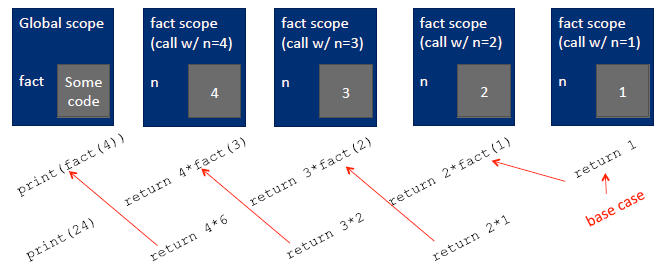
\includegraphics[width=0.6\textwidth]{figs/recursion/recursion-factorial-scope.png}
\end{figure}

\end{frame}

% Observaciones acerca de los algoritmos recursivos
\begin{frame}[fragile]{Recursividad: observaciones}
    \begin{itemize}
        \item Cada llamada a una función recursiva {\blue\bfseries crea su propio scope/ambiente}.
        
        \item Las asignaciones de variables en un ambiente no son afectadas por una llamada recursiva\footnote{\small Al utilizar el mismo nombre de variable, pero son objetos diferentes en ambientes separados}.
        
        \item El flujo de control regresa al {\orange\bfseries ambiente previo} cuando la llamada a la función retorna su valor.
    \end{itemize}
\end{frame}

% Iteración vs. Recursión
\begin{frame}[fragile]{Iteración vs. Recursión}
    \begin{columns}
        \begin{column}{0.5\textwidth}
\begin{lstlisting}[basicstyle=\linespread{1}\footnotesize\ttfamily]
def factorial_iter(n):
    prod = 1
    for i in range(1, n+1):
        prod *= i
    return prod
\end{lstlisting}
        \end{column}
        \begin{column}{0.5\textwidth}
\begin{lstlisting}[basicstyle=\linespread{1}\footnotesize\ttfamily]
def factorial_rec(n): 
    if n == 1:
        return 1 
    else:
        return n * factorial_rec(n-1)
\end{lstlisting}        
        \end{column}
    \end{columns}
    
    \begin{itemize}
        \item La recursión puede ser más simple, más intuitiva.
        \item La recursión {\orange puede ser más eficiente} desde el punto del programador.
        \item Puede {\orange no ser tan eficiente} desde el punto de visa de la computadora.
    \end{itemize}
\end{frame}

% Razonamiento inductivo
\begin{frame}[fragile]{Razonamiento inductivo}
    \begin{columns}
        \begin{column}{0.5\textwidth}
            \begin{itemize}
                \item ¿Cómo sabemos que nuestro código recursivo funcionará?
                
                \item \lstinline|mult_iter| termina, porque \lstinline|b| es inicialmente positivo y decrece en cada iteración, hasta que eventualmente \lstinline|b < 0|.
                
                \item \lstinline|mult| llamado con \lstinline|b=1| es el caso {\blue base}.
                
                \item \lstinline|mult| llamada con  \lstinline|b>1| hace una llamada recursiva con \lstinline|b| más pequeño $\Rightarrow$ eventualmente se llamará con \lstinline|b=1|.
            \end{itemize}
        \end{column}
        \begin{column}{0.5\textwidth}
\begin{lstlisting}
def mult_iter(a, b): 
    result = 0
    while b > 0: 
        result += a
        b -= 1
    return result

def mult(a, b):
    if b == 1:
        return a
    else:
        return a + mult(a, b-1)
\end{lstlisting}
        \end{column}
    \end{columns}
\end{frame}

% Inducción matemática
\begin{frame}[fragile]{Inducción matemática}
    \begin{itemize}
        \item Recordemos la {\orange\bfseries inducción matemática}: 1) asumimos $P_1$, luego probamos $P_n \Rightarrow P_{n+1}$.
        
        \item La misma lógica aplica:
\begin{lstlisting}
def mult(a, b):
    if b == 1:
        return a
    else:
        return a + mult(a, b-1)
\end{lstlisting}

        \item Para el {\orange caso base}, mostramos que \lstinline|mult| devuelve un valor correcto.
        
        \item Para el caso recursivo, asumimos que \lstinline|mult| retorna correctamente respuestas para problemas con más pequeños que \lstinline|b|, por lo tanto, también lo hace para problemas de tamaño \lstinline|b|.

        \item Por inducción, el código devuelve respuestas correctas.
    \end{itemize}
\end{frame}

\subsection{Torres de Hanoi}
% Torres de Hanoi
\begin{frame}[fragile]{Torres de Hanoi}
    \begin{itemize}
        \item 3 postes verticales.
        \item Pila de discos de diferentes tamaños en uno de los postes.
        \item Se deben mover hacia otro poste. En este caso, ¡el universo termina!
        \item {\blue\bfseries Reglas:} solamente se puede mover 1 disco a la vez y un disco más grande no puede cubrir a un disco más pequeño.
    \end{itemize}
    \begin{figure}
        \centering
        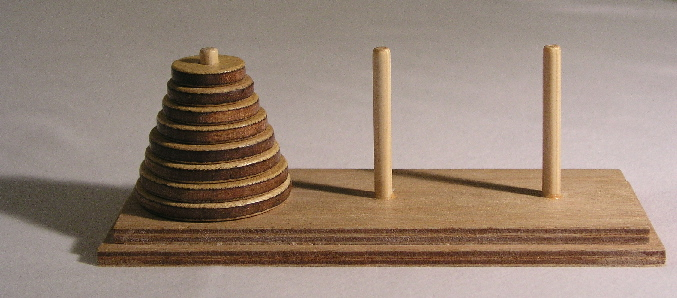
\includegraphics[width=0.6\textwidth]{figs/recursion/hanoi-towers.jpeg}
    \end{figure}
\end{frame}

\begin{frame}[fragile]{Torres de Hanoi}
    \begin{itemize}
        \item Habiendo visto algunos ejemplos, ¿cómo escribimos un programa para imprimir el conjunto de movimientos correctos?
        
        \item Debemos {\orange\bfseries ¡pensar recursivamente!}
        \begin{itemize}
            \item Resolver un problema más pequeño y más básico.
        \end{itemize}
    \end{itemize}
\end{frame}

% Código de torres de Hanoi
\begin{frame}[fragile]{Torres de Hanoi}
\begin{lstlisting}
def printMove(fr, to):
    print('move from ' + str(fr) + ' to ' + str(to))

def Towers(n, fr, to, spare):
    if n == 1:
        printMove(fr, to)
    else:
        Towers(n-1, fr, spare, to)
        Towers(1, fr, to, spare)
        Towers(n-1, spare, to, fr)
\end{lstlisting}
\end{frame}

\subsection{Fibonacci}
% Recursión con múltiples casos base
\begin{frame}[fragile]{Recursión con múltiples casos base}
    Leonardo de Pisa (Fibonacci) modeló el siguiente reto: 
    \begin{itemize}
        \item Un par de conejos recién nacidos (una hembra y un macho) se ponen en un corral
        \item Los conejos se aparean a la edad de un mes
        \item Los conejos tienen un período de gestación de un mes
        \item Suponga que los conejos nunca mueren, que la hembra siempre produce un nuevo par (un macho, una hembra) cada mes desde su segundo mes en adelante.
        \item ¿Cuántas conejas hay al final de un año?
    \end{itemize}
\end{frame}

% Diapositivas con conejos
\includeslides{22-31}{slides-60001/MIT6_0001F16_Lec6_mod.pdf}{Fibonacci}

\begin{frame}[fragile]{Fibonacci}
    \begin{itemize}
        \item Sucesión de eventos:
        \begin{itemize}
            \item Luego de un mes --- 1 hembra.
            \item Luego de un segundo mes --- 1 hembra (ahora preñada).
            \item Al tercer mes - 2 hembras, una preñada y otra no.
        \end{itemize}
        
        \item En general, $f(n) = f(n-1) + f(n-2)$: \begin{itemize}
            \item Cada hembra viva en $n-2$ produce una hembra en el mes $n$.
            \item Estas se suman a las hembras en el mes $n-1$.
        \end{itemize}
    \end{itemize}
\end{frame}

\begin{frame}[fragile]{Fibonacci}
    \begin{itemize}
        \item {\blue\bfseries Casos base}: $f(0)=1$ y $f(1)=1$.
        \item {\blue\bfseries Caso recursivo}: $f(n) = f(n-1) + f(n-2)$.
    
\begin{lstlisting}
def fib(x):
    """assumes x an int >= 0
       returns Fibonacci of x"""
    if x == 0 or x == 1:
        return 1
    else:
        return fib(x-1) + fib(x-2)
\end{lstlisting}

        \item \href{http://pythontutor.com/visualize.html#code=def%20fib%28x%29%3A%0A%20%20%20%20%22%22%22assumes%20x%20an%20int%20%3E%3D%200%0A%20%20%20%20%20%20%20returns%20Fibonacci%20of%20x%22%22%22%0A%20%20%20%20if%20x%20%3D%3D%200%20or%20x%20%3D%3D%201%3A%0A%20%20%20%20%20%20%20%20return%201%0A%20%20%20%20else%3A%0A%20%20%20%20%20%20%20%20return%20fib%28x-1%29%20%2B%20fib%28x-2%29%0A%20%20%20%20%20%20%20%20%0Aprint%28fib%284%29%29&cumulative=false&curInstr=38&heapPrimitives=nevernest&mode=display&origin=opt-frontend.js&py=3&rawInputLstJSON=%5B%5D&textReferences=false}{Ver en Python Tutor}
    \end{itemize}
\end{frame}

% Palíndromos
\subsection{Palíndromos}
\begin{frame}[fragile]{Palíndromos}
    \begin{itemize}
        \item ¿Cómo revisamos si un \textit{string} es un palíndromo (se lee igual al derecho y al revés).
        
        \item Primero, obtenemos los caracteres: 
        \begin{itemize}
            \item Quitamos puntuación.
            \item Ajustamos mayúsculas y minúsculas
        \end{itemize}
        
        \item Luego: 
        \begin{itemize}
            \item {\orange\bfseries Caso base:} \textit{string} de largo 0 o 1 es palíndromo.
            \item {\orange\bfseries Caso recursivo:} si primer y último caracter coinciden, es palíndromo si la sección del centro es palíndromo.
        \end{itemize}
    \end{itemize}
\end{frame}

% Ejemplo palíndromo
\includeslides{37}{slides-60001/MIT6_0001F16_Lec6_mod.pdf}{Palíndromo}

\begin{frame}[fragile]{Palíndromo}

\begin{lstlisting}
def isPalindrome(s):

    def toChars(s):
        s = s.lower()
        ans = ''
        for c in s:
            if c in 'abcdefghijklmnopqrstuvwxyz':
                ans = ans + c
        return ans

    def isPal(s):
        if len(s) <= 1:
            return True
        else:
            return s[0] == s[-1] and isPal(s[1:-1])

    return isPal(toChars(s))
\end{lstlisting}
\end{frame}

% Concepto de divide y conquistarás
\begin{frame}[fragile]{Divide y conquistarás}
    \begin{itemize}
        \item Este es también un ejemplo de la estrategia {\blue\bfseries divide y conquistarás}. 
        
        \item Podemos resolver un problema {\orange difícil} descomponiéndolo en partes tales que:
        \begin{itemize}
            \item Los {\orange\bfseries subproblemas son más fáciles de resolver}.
            \item Las soluciones a los subproblemas se pueden {\orange\bfseries combinar} para resolver el problema original.
        \end{itemize}
    \end{itemize}
    \begin{figure}
        \centering
        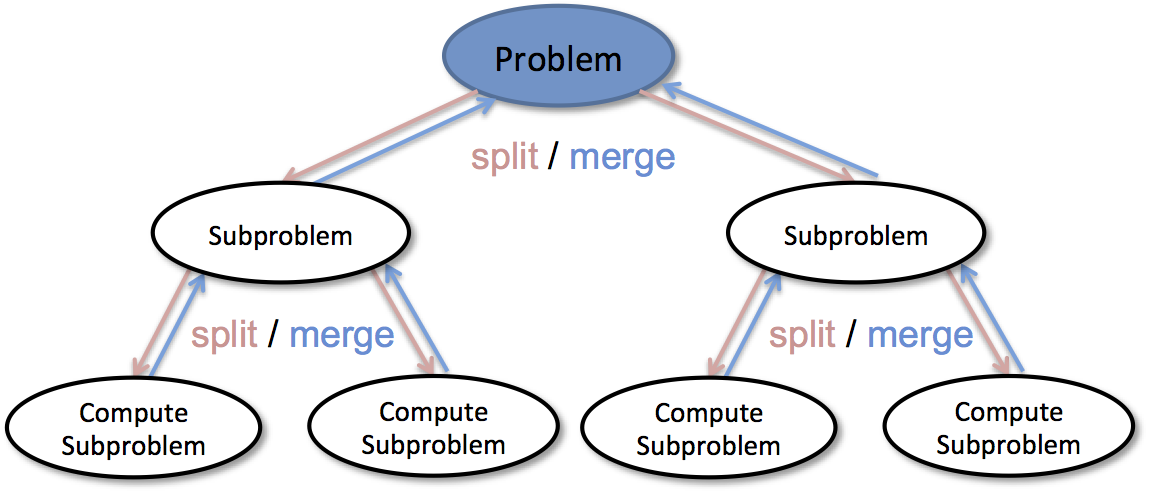
\includegraphics[width=0.8\textwidth]{figs/recursion/divide-and-conquer.png}
    \end{figure}
\end{frame}

% Ejercicios
\begin{frame}[fragile]{Ejercicio}
    \begin{itemize}
        \item Escribir una función recursiva que implemente el algoritmo de Euclides para encontrar el \emph{máximo común divisor} (mcd) de dos números $a$ y $b$.
        
        \item ¿Cuál es el caso base?
        
        \item ¿Cuál es el paso recursivo?
        
        \item Tip: busque el vídeo de \emph{Derivando} en Youtube para guiarse con la solución.
    \end{itemize}
\end{frame}

% Ejemplo de recursividad con fibonacci y diccionarios
% Quizás esto va después de ver recursión simple
\includeslides{54-57}{slides-60001/MIT6_0001F16_Lec6_mod.pdf}{Eficiencia: Fibonacci con diccionarios}



%-----------------------------------------------------------------
% Termina el contenido de la presentación
%-----------------------------------------------------------------

\begin{comment}

% Slide with two columns, half and half
\begin{frame}[fragile]{}
    \begin{columns}
        \begin{column}{0.5\textwidth}
        \end{column}
        \begin{column}{0.5\textwidth}
        \end{column}
    \end{columns}
\end{frame}

% Slide with bullets
\begin{frame}[fragile]{}
    \begin{itemize}
        \item 
    \end{itemize}
\end{frame}

% Slide with bullets and code
\begin{frame}[fragile]{}
    \begin{itemize}
        \item 
    \end{itemize}
\begin{lstlisting}
Code goes here
\end{lstlisting}
\end{frame}

% Include PDF 
\setbeamercolor{background canvas}{bg=}
\includepdf[pages=541-542, link=true, fitpaper]{slides-60001/MIT6_0001F16_Lec4.pdf}

% Include PDF slides with title
\setbeamercolor{background canvas}{bg=}
\includepdf[pages={21-22}, link=true, pagecommand={%
\Large\blue\bfseries\underline{%
Título de las diapositivas\phantom{g}}%
\vspace{-1em}%
\vskip 1.0mm}]{slides-60001/MIT6_0001F16_Lec4_mod.pdf}

% Pytutor
\href{URL}{Ver en Python Tutor}


\end{comment}

\end{document}